\documentclass[12pt]{scrartcl}
\usepackage{graphicx}
\usepackage{amsmath}

\begin{document}

%Title section

\titlehead{CS department, Technion}
\subject{Introduction to Optimization and Deep Learning 236330}
\title{HW 3}
\subtitle{Quasi-Newton BFGS method and DNN training}
\author{Uri Kirstein 311137095 \hfill sukirstn@campus.technion.ac.il\and Pavel Rastopchin 321082026 pavelr@campus.technion.ac.il}
\date{\today}
\maketitle

 %end of title section
\section*{Part 1 - BFGS}
\subsection*{Task 2}
We chose $N=10$. Our starting point was $x_0=(0,0,..0)$. We know that a local minimum of the function exists at $x^*=(1,1,...)$ and that $p^*=0$ (our function is non-negative so this must be a global minimum as well). We stopped after 60 iterations (we started from iteration number 0) at
\begin{center}
$x_{final}$ =[ 1.,  1., 1., 1., 1., 1., 1., 1., 1., 1.]
\end{center}
The error function and gradient at this point is $$f(x_{final})-p^*\approx 0$$
$\nabla f(x_{final})=$[-1.03489194e-07 4.64227620e-07 -2.33440170e-07 -3.37145026e-07 \\
4.63302603e-07 1.27499791e-07 -6.70338432e-07 5.13097599e-07 -3.48798911e-07 \\
1.10922516e-07]
$$||\nabla f(x_{final})|| = 1.2132069569224647e-06$$
We can see in the graph below that the error function $f(x_k)-p^*$, where $k$ is the number of iterations, is monotonously decreasing. This means we always advance in the direction of the minimum.
\begin{figure}[ht!]
	\hfill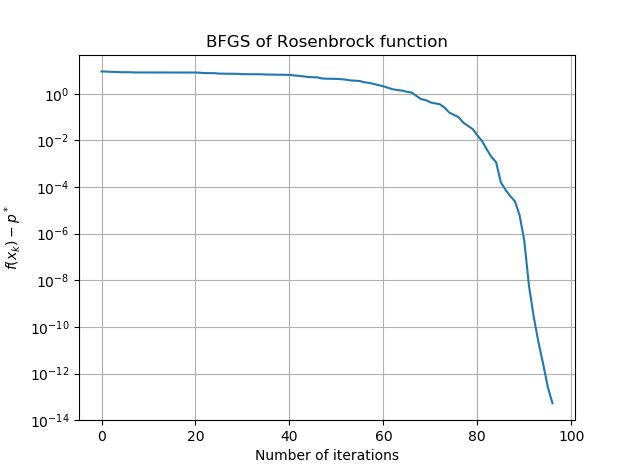
\includegraphics[width=\linewidth]{rosenbrock_graph.jpg}\hspace*{\fill}
	\caption{Task 2}
\end{figure}

\section*{Part 2 - Deep Neural Network}
\subsection*{Task 3}
\begin{align*}
\Psi(r_i)&=r_i^2\\
&=[F(x^i,w)-y_i]^2\\
&=\{w_3^T\phi_2[w_2^T\phi_1(w_1^Tx^i+b_1)+b_2]+b_3 -x_1^i exp[-(x_1^i)^2-(x_2^i)^2]\}^2
\end{align*}
We will use the following derivative:
$$\frac{d}{dx}\phi_1=\frac{d}{dx}\phi_2=\frac{d}{dx}tanh(x)=
\frac{1}{cosh^2(x)}$$
Using the chain rule:
\begin{align*}
\nabla_{w_1}\Psi %= \frac{\partial}{\partial w_1}r_i^2 //
%= 2r_i\frac{\partial}{\partial w_1}r_i
\end{align*}

\begin{center}
\boxed{\nabla_{b_3}\Psi = 1}
\end{center}

\end{document}
